% Definitions for this chapters figures.
\def\layerseptikznn{2.5cm}

This chapter discusses the background to several topics used throughout our work. We start by introducing the original artificial ant trail problem proposed by Jefferson and Koza. Next, we will discuss a model for biological neurons, the perceptron. The perceptron is used as the computational unit in the larger networks that perform computations to form \glspl{ann}. Then, we discuss the use of \glspl{ga} as a means to optimize the function of preceptrons.  A discussion on \glspl{crn} concludes this background chapter.

\section{Trail Problems}
\label{sec:trail_problems_bg}
Jefferson \textit{et al.} introduced the trail navigation problem in~\cite{Jefferson1992-ph}. In this task, an artificial ant is placed in a $32 \times 32$ grid. The goal is for the ant to collect as many pieces of food on the trail in a limited number of moves. Figure~\ref{fig:johnmuirtrailimage} shows the original John Muir trail proposed by Jefferson. The trail is toroidal, meaning that the top row of the trail is adjacent to the bottom row and the left and right rows are also adjacent. Starting in the top-left corner facing right, the only input the ant receives is if there is food placed directly in front of the space that the ant is facing.

The ant makes a decision for the next action based off the only input of if there is food ahead. The actions that the ant can take are move forward, turn left, turn right, or do nothing. Taking any of these four actions (including turns) counts as a move. As as an example, turning left followed by a forward more is two moves. The score of the ant is measured by the number of pieces of food it consumes within a limited number of moves, which was 200 in Jefferson's work. After an ant steps on a piece of food, that food is considered ``consumed'' so that it only receives credit for navigating over that part of the trail one time. The trail gets progressively more difficult adding gaps of increasing length and additional turns. Jefferson and Koza both designed an initial system and then evolved the parameters on it to search for an optimal control system.

\begin{figure}[tbp]
\centering
\includegraphics[width=0.9\textwidth]{john_muir_trail}
\caption[John Muir Trail]{The original John Muir trail proposed by Jefferson~\cite{Jefferson1992-ph}. This trail is a $32 \times 32$ toroidal grid and contains 89 pieces of food (represented by squares with circles in them). The ant is represented by an arrow in the top left corner (0, 0) facing to the right. The shaded squares that are empty are visual aids to indicate the optimal path proposed by Jefferson.}
\label{fig:johnmuirtrailimage}
\end{figure}

Jefferson's work tested the decision making capability of the ant through \glspl{fsm} and \glspl{ann}. These \glspl{fsm} were hand-designed initially and then later evolved to search for a better solution with a \gls{ga}. Using \glspl{fsm}, the authors found that a simple four state \gls{fsm} could get a score of 42 in 200 moves. Adding a single state (to form a five-state \gls{fsm}) allowed the \gls{fsm} to achieve a score of 81 in 200 time steps. Given more time, Jefferson found it actually consumed all of the food in 314 time steps. After 100 generations, Jefferson found the ``Champ-100'' \gls{fsm} that was capable of scoring an 89 (max score) through \glspl{ga}.

Using the same \gls{ga} configuration as the \gls{fsm}, an \gls{ann} capable of scoring the maximum of 89 was found in generation 94 by Jefferson. The network they used was a recurrent \gls{ann} with two input perceptrons, five hidden units, and four output units. Figure~\ref{fig:jefferson_original_nn} shows the recurrent \gls{ann}. The network featured two input perceptrons, a single hidden layer with five hidden perceptrons, and an output layer with four perceptrons. The neurons were fully forward connected, including a connection from the input layer to the output layer. Additionally, there is a recurrent connection from the hidden layer back to itself. The two inputs indicated if there was food ahead and the other was an inverse of the first. This is necessary since the \gls{ann} would not activate with just an input of 0 in the case of no food. The four output neurons were compared and the one with the largest output would determine the move.

\begin{figure}
\centering
\begin{tikzpicture}[->,draw=black!100, node distance=\layerseptikznn]
    % Based off code form http://www.texample.net/tikz/examples/neural-network/
    \tikzstyle{every pin edge}=[<-,shorten <=1pt]
    \tikzstyle{neuron}=[circle,draw=black!50,fill=white!25,minimum size=25pt,inner sep=0pt]
    \tikzstyle{input neuron}=[neuron, draw=black!50, fill=Accent-4-1];
    \tikzstyle{output neuron}=[neuron, draw=black!50, fill=Accent-4-2];
    \tikzstyle{hidden neuron}=[neuron, draw=black!50, fill=Accent-4-3];
    \tikzstyle{annot} = [text width=4em, text centered]

    % Draw the input layer nodes
    \node[input neuron, pin=left:Food] (I-1) at (0,-2) {};
    \node[input neuron, pin=left:No Food] (I-2) at (0,-3) {};

    % Draw the hidden layer nodes
    \foreach \name / \y in {1,...,5}
        \path[yshift=0.5cm]
            node[hidden neuron] (H-\name) at (\layerseptikznn, -\y) {H\name};

    % Draw the output layer node
        \path node[output neuron, pin={[pin edge={->}]right:None}] 
                (O-1) at (\layerseptikznn * 2, -1) {};
        \path node[output neuron, pin={[pin edge={->}]right:Forward}] 
                (O-2) at (\layerseptikznn * 2, -2) {};
        \path node[output neuron, pin={[pin edge={->}]right:Left}] 
                (O-3) at (\layerseptikznn * 2, -3) {};
        \path node[output neuron, pin={[pin edge={->}]right:Right}] 
                (O-4) at (\layerseptikznn * 2, -4) {};

    % Connect every node in the input layer with every node in the
    % hidden layer.
    \foreach \source in {1,...,2}
        \foreach \dest in {1,...,5}
            \path (I-\source) edge (H-\dest);
            
    \draw[-, draw=brown!100, thick](I-1) -- ($ (I-1) !.75! (O-2) $);
    \draw[-, draw=violet!100, thick](I-2) -- ($ (I-2) !.75! (O-3) $);
            
    \foreach \dest in {1,...,4}{
        \draw[->, draw=brown!100] ($ (I-1) !.75! (O-2) $) -- (O-\dest.west);
        \draw[->, draw=violet!100] ($ (I-2) !.75! (O-3) $) -- (O-\dest.west);
    }

    % Connect every node in the hidden layer with the output layer
    \foreach \source in {1,...,5}
        \foreach \dest in {1,...,4}
            \path (H-\source) edge (O-\dest);

    % Annotate the layers
    \node[annot,above of=H-1, node distance=1cm] (hl) {Hidden layer};
    \node[annot,left of=hl] {Input layer};
    \node[annot,right of=hl] {Output layer};
\end{tikzpicture}
\caption[Jefferson John Muir Trail ANN]{The \gls{ann} used by Jefferson in. This recurrent \gls{ann} features two input (that are the inverse of each other), five hidden, and four output units. Each of the four outputs represents an action the agent can take. The recurrent network features connections from the hidden layer back to itself (e.g., H1 back into H1) that are not shown to reduce clutter.}
\label{fig:jefferson_original_nn}
\end{figure}

Koza expanded Jefferson's work by studying the artificial ant navigating through the Santa Fe Trail~\cite{Koza1992-xs}. According to Koza, the Santa Fe trail is a more difficult trail and is shown in Figure~\ref{fig:santa_fe_trail_image}. The actions and task are the same as Jefferson's John Muir trail. Koza also performed analysis using evolving LISP programs instead of \glspl{ann} or \glspl{fsm} like Jefferson. With the evolving LISP programs, Koza found a solution scoring the maximum (89) in generation 21.

\begin{figure}[tbp]
\centering
\includegraphics[width=0.9\textwidth]{santa_fe_trail}
\caption[Santa Fe Trail]{The Santa Fe Trail proposed by Koza~\cite{Koza1992-xs}. This trail (like the John Muir Trail, Figure~\ref{fig:johnmuirtrailimage}) is $32 \times 32$ and toroidal. The trail contains 89 pieces of food (same as trail segments in Jefferson) and are represented by squares with circles in them here. Shaded squares are provided as a visual aid to indicate the optimal route proposed by Koza. The ant is an arrow in the top left corner facing to the right.}
\label{fig:santa_fe_trail_image}
\end{figure}

Koza's work on the Santa Fe trail has created an entire new field of research with the optimization of evolution of these programs, also known as \gls{gp}. As a result, thee Santa Fe trail tends to be a more popular trail for analysis in recent research. Doucette and Heywood present an improved novelty-based fitness algorithm that they then tested against the Santa Fe trail~\cite{Doucette2010-yc}. Christensen and Oppacher presented a set of trees that efficiently search the solution space of Koza's \glspl{gp} requiring less computational power~\cite{Christensen2007-vj}. The Santa Fe trail has also been used as a basis to prove implementation in reservoir computing~\cite{Gargesa2013-rx}.

The use of a \gls{fsm} or \gls{gp} seem to dominate the recent literature that we have found for directly solving the trail problem. Wilson and Kaur work on a \gls{gp} representation and a modified function to improve the rate at which the system learns the task~\cite{Wilson2013-vt}. The authors develop a more effective \gls{gp} to solve the problem by evaluating and improving the fitness landscape.

Chivilikhin \textit{et al.} extend Wilson and Kaur's work with their new algorithm (MuACO\textit{sm}) that performs well at the task of optimizing the \gls{fsm} implementation~\cite{Chivilikhin2013-sw}. Other improvements on the implementations using Koza's LISP programs were performed by Christansen and Oppacher~\cite{Christensen2007-vj} and Karmin and Ryan~\cite{Karim2012-ik}. The algorithms for solving the trail problem we have discussed thus far are aimed more towards improving the \gls{fsm} or \gls{gp} implementations.

Silva \textit{et al.} published work that discusses a hybrid combination of \gls{ann} and \gls{gp} to form what they call a \gls{gpn}~\cite{Silva1999-kw}. In a \gls{gpn}, the structure is laid out similar to what you would find in a \gls{ann}, but rather than have the nodes do processing that you would typically find in an \gls{ann} (like a perceptron), they are modeled by a specific program. So from an architectural layout, they follow \glspl{ann}, but the transfer function of each node is actually more akin to a \gls{gp}. The authors prove functionality by consuming all pieces of food on the Santa Fe trail with a \gls{gpn}.

The \gls{ann} implementation lends itself well for applications that may not have the robust architecture or infrastructure necessary to implement such solutions. One such field is the use of chemistry to solve this problem. First, we will discuss an explanation into perceptrons and the \gls{ann} that formed Jefferson's solution to the John Muir trail.

\section{Perceptrons and Artificial Neural Networks}
McCulloch and Pitts were the pioneers of the field with their early models of neurons~\cite{McCulloch1943-li}. They presented a basic model to represent a neuron based off biological systems. Combining several of these neurons and connecting them together forms a basic \gls{ann}. Since the original work by McCulloch and Pitts, others have developed more refined models of neurons.

One such model is the perceptron presented by Rosenblatt~\cite{Rosenblatt1958-yq} and later refined by Minsky and Papert~\cite{Minsky1987-zx}. The perceptron can act as a binary classifier. An example binary classification perceptron has multiple inputs that are transformed to one or more outputs. Each of these outputs would get converted to a binary value, such as $0$ and $1$, if a specified bias is met. Each of the input connections has an associated weight that determines the relative strength of that input to a different input~\cite{Rojas1996-yd}. Figure~\ref{fig:preceptron_example} shows a perceptron with three inputs and a single output.

\begin{figure}[ht]
\centering
\begin{tikzpicture}[shorten >=1pt,->,draw=black!50]
    \tikzstyle{neuron}=[circle,draw=black!50,fill=white!25,minimum size=25pt,inner sep=0pt]
    \tikzstyle{input neuron}=[neuron, draw=black!50, fill=Accent-4-4];
    \tikzstyle{annot} = [text width=4em, text centered]
    
    \node[annot] (theta) at (0, 0) {$\theta$};
    \node[annot, below of=theta] (x1) {$x_1$};
    \node[annot, below of=x1] (x2) {$x_2$};
    \node[annot, below of=x2] (x3) {$x_3$};

    \node[input neuron, right=2.5cm of x1 |- x2, align=center] (P1) {Perceptron \\ $\theta$};
    
    \node[annot, right=2.5cm of P1] (y) {$Y$};
    
    \draw[->,thick] (theta) -- (P1) {};
    \draw[->,thick] (x1) -- (P1) node [midway, below] {$w_1$};
    \draw[->,thick] (x2) -- (P1) node [midway, below] {$w_2$};
    \draw[->,thick] (x3) -- (P1) node [midway, below] {$w_3$};
    
    \draw[->,thick] (P1) -- (y) {};
    

\end{tikzpicture}
\caption[Diagram of Three Input Perceptron]{A model of a binary threshold perceptron with three inputs. This particular perceptron multiplies the weights ($w_n$) by each corresponding input ($x_n$). If the sum of these values exceeds a bias value ($\theta$), the output ($Y$) is $1$, otherwise, it is $0$.}
\label{fig:preceptron_example}
\end{figure}

The perceptron in Figure~\ref{fig:preceptron_example} takes three input values, $x_1$, $x_2$, and $x_3$ to perform a binary classification to the output, $Y$. Equation~\ref{eq:percept_ouptut} shows the function that classifies a perceptron with $n$ inputs.

\begin{equation} \label{eq:percept_ouptut}
Y = 
    \begin{cases}
        1, & \text{if}\ (\sum\limits_{i=1}^n  x_i  w_i) - \theta > 0\\
        0, & \text{otherwise}
    \end{cases}
\end{equation}

Perceptrons typically contain a bias, represented by $\theta$, that allows is the adjustment for the threshold point. In other words, if the sum of the weights is not greater than the bias, then this perceptron's output will result in 0. 

Perceptrons can act as more than just binary classifiers. Perceptrons can also behave in an analog fashion where the output is any range of values~\cite{Rosenblatt1958-yq}. For example, rather than assigning the values to binary values, they could map to values on a step, sigmoid, or hyperbolic tangent function~\cite{Rojas1996-yd} to perform a desired transformation that may translate closer to the behavior of biological neurons.

The weights on the perceptron are user definable, but this is generally impractical when connecting several perceptrons together to form a larger network. One way the weights are set is by a process known as learning. In learning, the weights of the perceptron are adjusted to obtain the desired output. A basic method to learn is to randomly generate a set of test vectors and map them to the desired output~\cite{Rojas1996-yd}. Then, run each of these test vectors through the perceptron. If the desired output is obtained, no action is necessary on the weights. If the output is not the expected output, then the weights are either increased or decreased in proportion to the error in an attempt to get closer to the desired result.

An alternative means to search for the weight values is through the use of \acrfull{ga}. Through the process of selecting the top performers, the weights are initially randomly set and the best performing weights are carried forward in an evolutionarily process. This type of process allows arrival at an optimal solution modeled after biological evolution rather than the user having to specify or search for values. For larger networks, this is even impractical. The weights on the networks of perceptrons later are optimized using \glspl{ga} which we will discuss in the next section.

Now, taking several of the perceptrons and connecting them together forms what is referred to as an \acrfull{ann}. An \gls{ann} is a system that connected together several of these perceptrons (or another neuron model) that can adapt to a particular task and elicit a desired response. An \gls{ann} is an alternative model for computation on information~\cite{Rojas1996-yd}. They are typically formed by connecting the output of one perceptron to the input of another. This cascading of the perceptrons forms what are referred to as layers. Recall the weights on each of a perceptron's inputs allows us to control the output, so by cascading these elements together, it is possible to form complex networks of perceptrons. A typical \gls{ann} may look like that in Figure~\ref{fig:example_ann_intro}. 

\begin{figure}[ht]
\centering
\begin{tikzpicture}[shorten >=1pt,->,draw=black!50, node distance=\layerseptikznn]
    % Based off code form http://www.texample.net/tikz/examples/neural-network/
    \tikzstyle{every pin edge}=[<-,shorten <=1pt]
    \tikzstyle{neuron}=[circle,draw=black!50,fill=white!25,minimum size=25pt,inner sep=0pt]
    \tikzstyle{input neuron}=[neuron, draw=black!50, fill=Accent-4-1];
    \tikzstyle{output neuron}=[neuron, draw=black!50, fill=Accent-4-2];
    \tikzstyle{hidden neuron}=[neuron, draw=black!50, fill=Accent-4-3];
    \tikzstyle{annot} = [text width=4em, text centered]

    % Draw the input layer nodes
    \foreach \name / \y in {1,...,2}
        \node[input neuron, pin=left:Input \#\y] (I-\name) at (0,-\y) {};

    % Draw the hidden layer nodes
    \foreach \name / \y in {1,...,3}
        \path[yshift=0.5cm]
            node[hidden neuron] (H-\name) at (\layerseptikznn, -\y) {H\name};

    % Draw the output layer node
    \foreach \name / \y in {1,...,2}
        \path
            node[output neuron, pin={[pin edge={->}]right:Output \#\y}] 
                (O-\name) at (\layerseptikznn * 2, -\y) {};

    % Connect every node in the input layer with every node in the
    % hidden layer.
    \foreach \source in {1,...,2}
        \foreach \dest in {1,...,3}
            \path (I-\source) edge (H-\dest);

    % Connect every node in the hidden layer with the output layer
    \foreach \source in {1,...,3}
        \foreach \dest in {1,...,2}
            \path (H-\source) edge (O-\dest);

    % Annotate the layers
    \node[annot,above of=H-1, node distance=1cm] (hl) {Hidden layer};
    \node[annot,left of=hl] {Input layer};
    \node[annot,right of=hl] {Output layer};
\end{tikzpicture}
\caption[Example Artificial Neural Network]{Example \gls{ann} with an input layer, single hidden layer, and output layer. Each layer has two, three, and two perceptrons, respectively.}
\label{fig:example_ann_intro}
\end{figure}

The \gls{ann} in Figure~\ref{fig:example_ann_intro} is composed of seven perceptrons in three layers. This example network is also known as a feedforward network where signals only propagate forward and there is effectively no tracking of state or previous values. A recurrent network is one with connections back to itself or somewhere else in the network~\cite{Rojas1996-yd}. This recurrence gives a \gls{ann} a form of memory storage of previous state information. Passing the present value back to the perceptron acts effectively as a length one memory into the previous calculation.

The hidden layer of an \gls{ann} is the levels that are between the input and output layer. Some networks may contain numerous hidden layers or none at all. The connections between the perceptrons have associated weights. For example, neuron $H1$ has one arrow coming from Input $\#1$ and Input $\#2$ that would each have an associated, unique weight. As the size of the network continues to grow, so does the complexity for determining the weights to appropriately accomplish a desired task. The weights of the network are adjusted by hand (for small networks), through use of a \gls{ga}, or also updated in some instances with a method known as backpropagation. In short, the method calculates an error from ideal output through the neural network and updates the weights in a way to attempt to arrive at a more accurate solution~\cite{Rumelhart1988-hm}.

The weights for the \glspl{ann} in this work are set using a \gls{ga} because it was the same method that Jefferson used when optimizing the \gls{ann} in the ant trail task. They are set randomly to start and then optimized through an evolutionary process. As discussed in the previous section, Jefferson conducted a similar process to arrive at the best weights for the \gls{ann}. Now, we will discuss \glspl{ga} in greater detail. 

\section{Genetic Algorithms}
\Acrfullpl{ga} are used to search for optimal solutions to the delay line and agent navigating through the trails. \Glspl{ga} were first proposed by Holland~\cite{Holland1962-uk}~\cite{Holland1975-di}. In this work, Holland outlined \glspl{ga} as a means to take biological adaptation and use it as a means to adapt and evolve systems in a computer. Holland's approach was more a mathematical one rather than attempting to target a specific applications for the use of \glspl{ga}~\cite{Mitchell1998-tw}. In the last few decades, \glspl{ga} have served as a method of optimization in countless applications such as control systems~\cite{Fleming2002-br}, image enhancement~\cite{Pal1994-zb}, and neural networks~\cite{Menczer1994-vx}.

A \Gls{ga} is a type of evolutionary computation meant to model the behavior of biological evolution through adaption~\cite{Baeck2000-co}. Like the biological counterparts, \Glspl{ga} are made up of a population and have a set of functions to model behaviors to obtain variation in future populations: selection, crossover (also refereed to as recombination~\cite{Mitchell1998-tw}), and mutation. By evaluating a population, producing offspring, evaluating the offspring, and repeating this cycle, a solution is derived where a population is adapted to solve our particular application.

A population is made up of individuals composed of chromosomes. Each chromosome is a set of values that provide variation in control for a system. Holland originally proposed chromosomes that are made up of bit strings; however, other work has shown that a makeup of real-valued parameters and LISP symbolic expressions are also viable representations~\cite{Baeck2000-co}. LISP symbolic expressions are a way to represent nested or recursive list of data based off the LISP programming language. Many of the problems that Koza solves in his text are represented by LISP symbolic expressions~\cite{Koza1992-xs}. For our work, the chromosomes are typically made up of arrays in floating point values which are functionally equivalent to a bit stream. As an example, the weights on inputs to the perceptrons making up the trail systems are represented by an array of floating point values that cause each individual to respond differently to a set of inputs.

The evaluation of performance of a individual is known as its fitness. In biological terms, this is the tendency of an individual to reproduce in an environment~\cite{Mitchell1998-tw}. In \Glspl{ga}, the fitness is calculated by observing the actual output of a chromosome compared to the ideal or objective output of the function~\cite{Baeck2000-co}. For instance, in the fitness of the delay line (discussed in section~\ref{sec:dl_results}), individuals are measured by taking the difference between the observed value on a delayed version of the input versus the actual copy of the input. 

Selection is the process of taking individuals with the higher fitness as a basis for forming offspring. There are several methods available for selection such as

\begin{description}
\item[proportional selection] generates offspring from individuals directly \\ proportional to their respective fitnesses~\cite{Holland1975-di};
\item[roulette wheel selection] assigns a probability distribution to population where the probability of selection is proportional to the fitness and then selects, one at a time, an individual from the pool~\cite{Baeck2000-co};
\item[tournament selection] selects a specified number of individuals randomly from the population, choose the individual with the highest fitness in this group (or tournament), and repeat as desired~\cite{Brindle1981-rh}~\cite{Goldberg1991-kr};
\item[rank-based selection] selects the desired number of individuals from the entire population based only off a ranking of their fitness~\cite{Baker1985-fw};
\item[$\bm{(\mu, \lambda)}$ selection] form an offspring basis by generating individuals for each member of the population through mutation and/or crossover and save a defined set of them for subsequent crossover~\cite{Schwefel1976-er};
\item[$\bm{(\mu + \lambda)}$ selection] similar to $\bm{(\mu + \lambda)}$ selection, but select the top performers from both the pool of offspring \textbf{and} population~\cite{Schwefel1976-er}.
\end{description}

Combining a method with elements of rank-based selection (showing preference towards higher fitnesses) adds elitism. Elitism is a means to carry forward  members with a high fitness either directly or as a basis to form a new set of offspring. Selection methods that combine more than one of these means are known as \glspl{moea}. An example of such an algorithm is NSGA-II by Deb \textit{et al.}~\cite{Deb2000-so}. NSGA-II builds an algorithm similar to $(\mu + \lambda)$ selection, but uses tournament selection in addition to determine the best individuals for later formation of the offspring.

Crossover is where individuals are combined to produce offspring. A couple of common means to perform crossover are $n$-point crossover and uniform crossover. An $n$-point crossover effectively splits the parents at $n$ points where genetic material is alternated to the two offspring from the two parents~\cite{De_Jong1975-wc}. While $n$ only must be greater than one, one is rarely used in practice where $n = 2$ is the commonly selected value~\cite{Baeck2000-co}. The uniform crossover~\cite{Ackley1987-xa}~\cite{Syswerda1989-go} traverses bit by bit down a parent and probabilistically determines if a crossover will occur at the current position. A $p_x = 0.5$ is a commonly selected value for uniform crossovers~\cite{Baeck2000-co}~\cite{Ackley1987-xa}.

The last \gls{ga} operation we will discuss here is mutation. Like selection and crossover, there are numerous works on just the discussion of mutation and its importance in \Glspl{ga}. There are algorithms that utilize \glspl{fsm}~\cite{Baeck2000-co}, parse trees~\cite{Angeline1996-no}, or k-opt from travelling salesman problem~\cite{Lin1973-tp}. Throughout this work, the basic mutation utilized is a basic mutation randomly selecting bits in an individual to get flipped~\cite{Mitchell1998-tw}. As a small example, you could have an individual represented by $0001$ that after mutation is $1001$ where the first bit was mutated.

There are a few ways that all of these steps get ordered to form a \gls{ga}. Also, varying the probability of each of the actions to occur will have an impact on how rapidly the population evolves. An example \gls{ga}, proposed by B\"{a}ck~\cite{Baeck2000-co}, may

\begin{enumerate}
\item initialize a population of individual chromosomes,
\item evaluate the population to calculate the fitness of the individuals,
\item \label{itm:ga_repeat_start} perform crossover,
\item mutate the population,
\item evaluate fitness,
\item select next members of population,
\item repeat from step~\ref{itm:ga_repeat_start} until desired number of generations are evaluated.
\end{enumerate}

Figure~\ref{fig:ga_flowchart_background} shows a flow chart of this particular \gls{ga}. Later on, we will discuss the genetic algorithms used to optimize the delay line and trail systems in section~\ref{sec:trail_runner_methods}. Now, with an understanding of the trail problem, how it was solved as an \gls{ann}, and how it was optimized with a \gls{ga}, we now shift focus to discuss \glspl{crn}. 

\begin{figure}
\centering
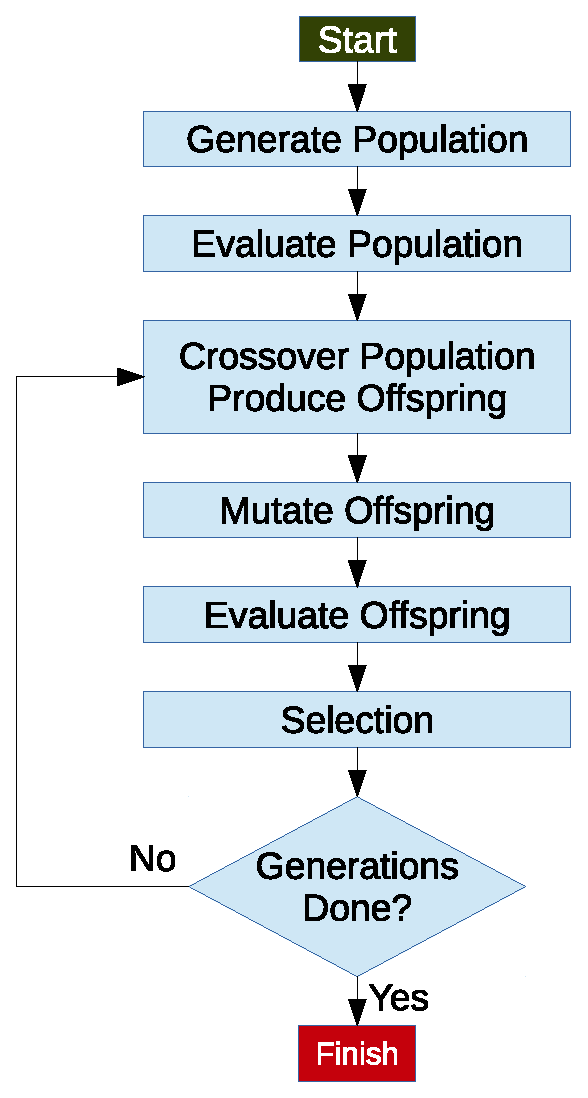
\includegraphics[width=0.5\textwidth]{ga_flowchart_background}
\caption[B\"{a}ck Simple Genetic Algorithm]{A simple genetic algorithm proposed by B\"{a}ck~\cite{Baeck2000-co}. This algorithm builds a population and then evaluates it. Next, it uses crossover to produce a pool of offspring and then mutates and evaluates the offspring. The best individuals are selected and this process is repeated until the specified number of generations are met.}
\label{fig:ga_flowchart_background}
\end{figure}

\section{Chemical Reaction Networks}
Portions of this section are borrowed from~\cite{Moles2014-ia}. The systems we use to model chemistry are known as \acrfullpl{crn}, which is an instance of an \acrfull{ac}~\cite{Dittrich2001-rn}. \Glspl{crn} give us a mean to model a set of chemical species and the way in which they react with each other to form new products. We model the chemistries by using several observations of nature, such as chemical kinetics and the law of conservation of mass. 

A \gls{crn} consists of a set of species and reactions with associated rates. In our system, molecular species are symbolic and unstructured, and there is no notion of space because we assume the solution is well stirred. In other words, the concentration of a given species is uniform throughout the solution and not unequally distributed. Actually, we do not need to handle the position of individual molecules, but rather transform all molecules of the same type (species) using rates generated by kinetic laws: mass-action~\cite{Horn1972-ob}~\cite{Erdi1989-ll} for regular and Michaelis\hyph Menten~\cite{Henri1903-jf}~\cite{Michaelis1913-zv}~\cite{Leskovac2003-ei} for catalytic reactions.

Dittrich~\cite{Dittrich2001-rn} describes an \gls{ac} made up of a finite set of molecular species and a finite set of reactions. The set of molecular species are represented by symbols. For example, the symbols representing the two reactants and products in our chemical example here are $S_1$, $S_2$, and $P$, respectively. The reactions are formed through multiple sets of species (reaction left side) that react to form products (reaction right side)~\cite{Banda2013-zs}. A reaction looks like $S_1 + S_2 \rightarrow P$ where reactants $S_1$ and $S_2$ form the product $P$.

We combine mass action kinetics with the ideas of \gls{ac} to express reaction rates for ordinary (non-catalytic) reactions. Epstein~\cite{Epstein1998-qw} expresses this through a series of differential equations. Given a generic chemical reaction $aS_1 + bS_2 \rightarrow cP$, the rate of reaction, $v$, is expressed by
\begin{equation}
v = -\frac{1}{a}\frac{d[S_1]}{dt} = -\frac{1}{b}\frac{d[S_2]}{dt} = \frac{1}{c}\frac{d[P]}{dt} = k[S_1]^a[S_2]^b,
\end{equation}
where $[S_1]$, $[S_2]$, and $[P]$ are the concentrations of the reactants, $S_1$ and $S_2$, and the product, $P$. Symbols $a$ and $b$ are stoichiometric constants, and $k$ is the reaction rate constant. Reactions could also be reversible, but in this paper, for simplification, we assume the reverse rate is always zero.

Michaelis-Menten kinetics describes the rate of a catalytic reaction where a substrate ($S$) is transformed into a product ($P$) through the use of an enzyme or catalyst ($E$) in a reaction modeled as $E + S \rightleftharpoons ES \rightarrow E + P$. The catalyst $E$ speeds up the rate of the reaction without being consumed in the process. The rate of a catalytic reaction is defined by
\begin{equation}
v = \frac{k_{cat}[E][S]}{K_m+[S]},
\end{equation}
where $k_{cat}$ and $K_m$ are rate constants~\cite{Copeland2004-sq}.

The simulations of \glspl{crn} were performed with \acrfull{coel}. \Gls{coel} is a tool developed by Banda \textit{et al.} that allows the simulation and evolution of \glspl{crn} using \glspl{ga}~\cite{Banda2014-qw}. The chemical simulations, as we will show later, take a longer period of time to run than a non-\gls{crn} simulation so distribution of the work across a \gls{hpc} cluster allows the simulations to execute faster. We have confidence in the results produced with multiple papers being published using the same tool. Building blocks, like perceptrons and \glspl{ann} as chemistries are also already modeled in \gls{coel}.

Various models of perceptrons that are constructed in a \glspl{crn} already exist. Banda \textit{et al.} have presented multiple models of the preceptron such as the \gls{asp}~\cite{Banda2014-bp} and \gls{aasp}~\cite{Banda2014-kg}. These two models of perceptrons both have a definition that allows direct mapping to a biological implementation. The \gls{aasp} is an improved version of the \gls{asp} that offers greater precision with a fewer number of reactions. Blount \textit{et al.} has shown that more than one of these pereceptrons, forming an \gls{ann}, in the same chemistry are possible with the use of chemical compartments~\cite{Blount_undated-ro}.

These chemical compartments are a means to isolate the reaction of a series of reactions from another set of reactions. From a modularity perspective, they also allow some sense of recursion by re-using the same species and reactions set by inserting multiple copies of the same compartment. Blount's compartments use a membrane to control the flow of interactions between each of the layers of an \gls{ann}. This gives way to allow multiple perceptrons to co-exist in the same solution without interfering with the processing of another perceptron. Now, in the next chapter, we will discuss the implementation of two different models of the delay line as a \gls{crn}.

